\begin{appendices}

	\chapter{Additional Figures}
	\label{app:additional_figures}

	% ------ DBSCAN and HDBSCAN Clustering ------
	\section{DBSCAN and HDBSCAN Clustering}
	\label{app:dbscan_hdbscan_clustering}

	\begin{figure}[H]
		\centering
		\begin{minipage}[t]{0.48\textwidth}
			\centering
			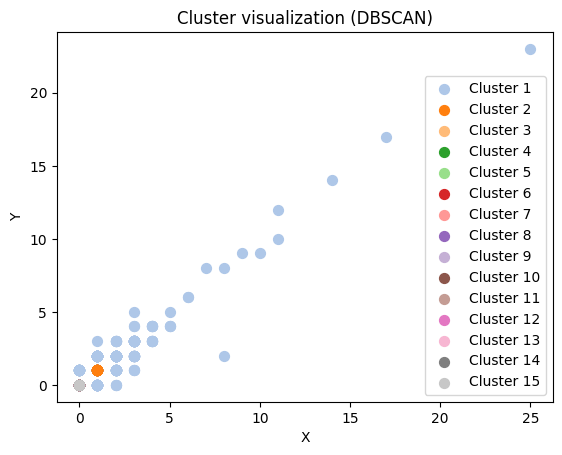
\includegraphics[width=0.95\textwidth]{../imgs/graphs/clustering/dbscan_nopca.png}
			\caption{Clusters obtained with DBSCAN after applying PCA.}
			\label{fig:clusters_dbscan_no_pca}
		\end{minipage}\hfill
		\begin{minipage}[t]{0.48\textwidth}
			\centering
			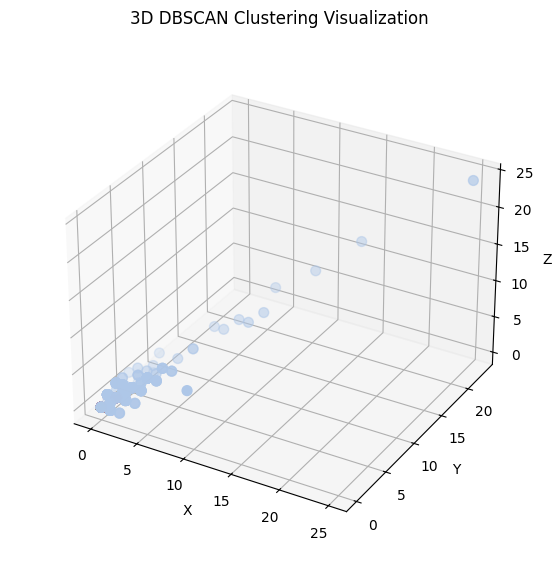
\includegraphics[width=0.95\textwidth]{../imgs/graphs/clustering/dbscan_nopca_3d.png}
			\caption{Clusters obtained with DBSCAN after applying PCA in 3D.}
			\label{fig:clusters_dbscan_no_pca_3d}
		\end{minipage}
	\end{figure}

	\begin{figure}[H]
		\centering
		\begin{minipage}[t]{0.48\textwidth}
			\centering
			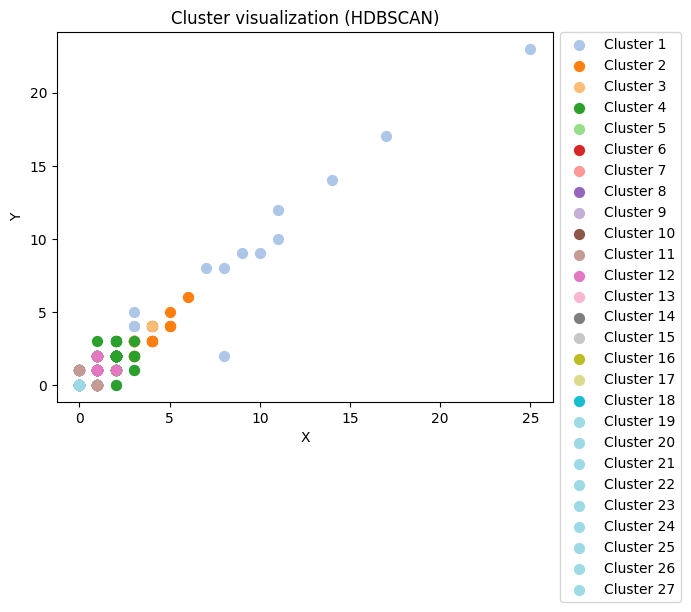
\includegraphics[width=0.95\textwidth]{../imgs/graphs/clustering/hdbscan_nopca.png}
			\caption{Clusters obtained with DBSCAN after applying PCA.}
			\label{fig:clusters_hdbscan_no_pca}
		\end{minipage}\hfill
		\begin{minipage}[t]{0.48\textwidth}
			\centering
			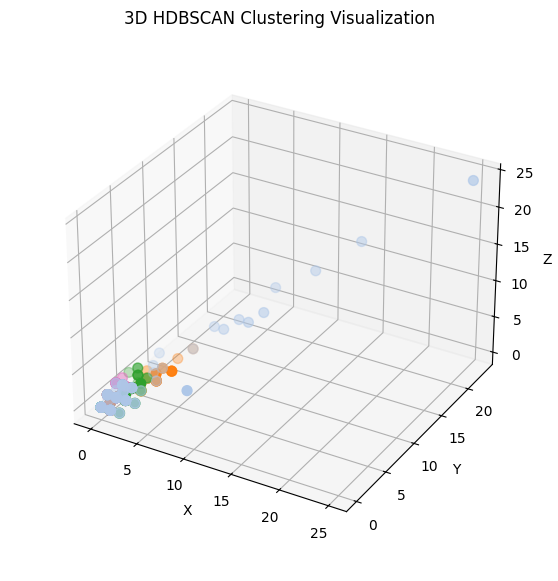
\includegraphics[width=0.95\textwidth]{../imgs/graphs/clustering/hdbscan_nopca_3d.png}
			\caption{Clusters obtained with DBSCAN after applying PCA in 3D.}
			\label{fig:clusters_hdbscan_no_pca_3d}
		\end{minipage}
	\end{figure}

	% ------ Initial CNN model performance ------
	\section{Initial CNN Model Performance}
	\label{app:initial_cnn_performance}

	\begin{figure}[H]
		\centering
		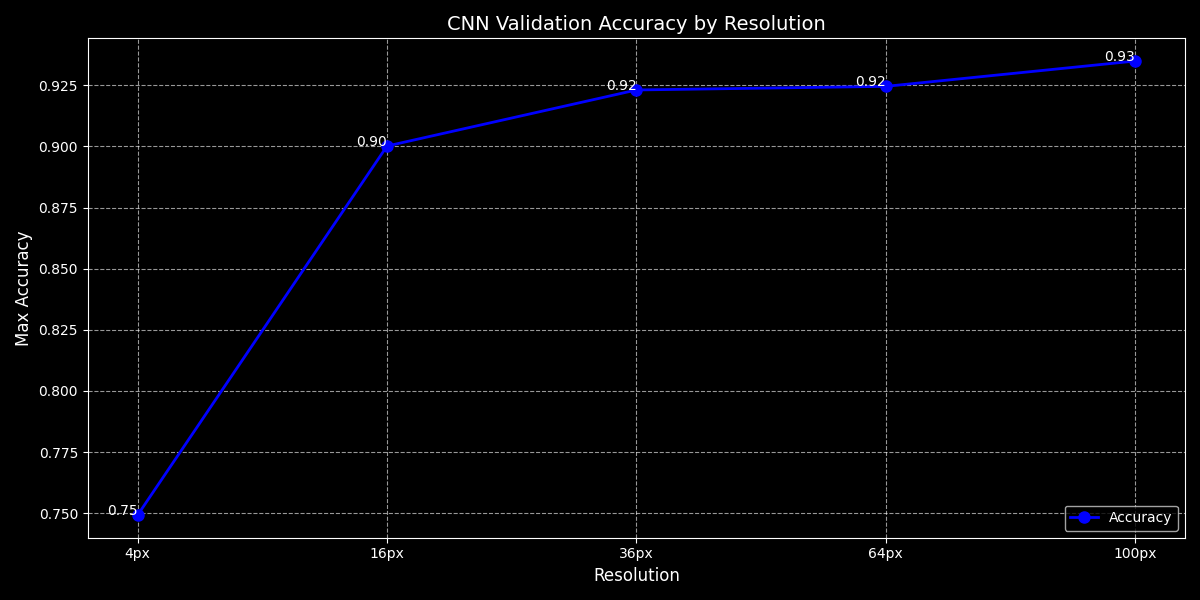
\includegraphics[width=0.65\textwidth]{../imgs/graphs/cnn_validation_accuracy_mosaics_line.png}
		\caption{Graph showing the validation accuracy of the CNN model on the mosaic images at 100px resolution without any
			additional techniques applied.}
		\label{fig:initial_accuracy_mosaic}
	\end{figure}

	\begin{figure}[H]
		\centering
		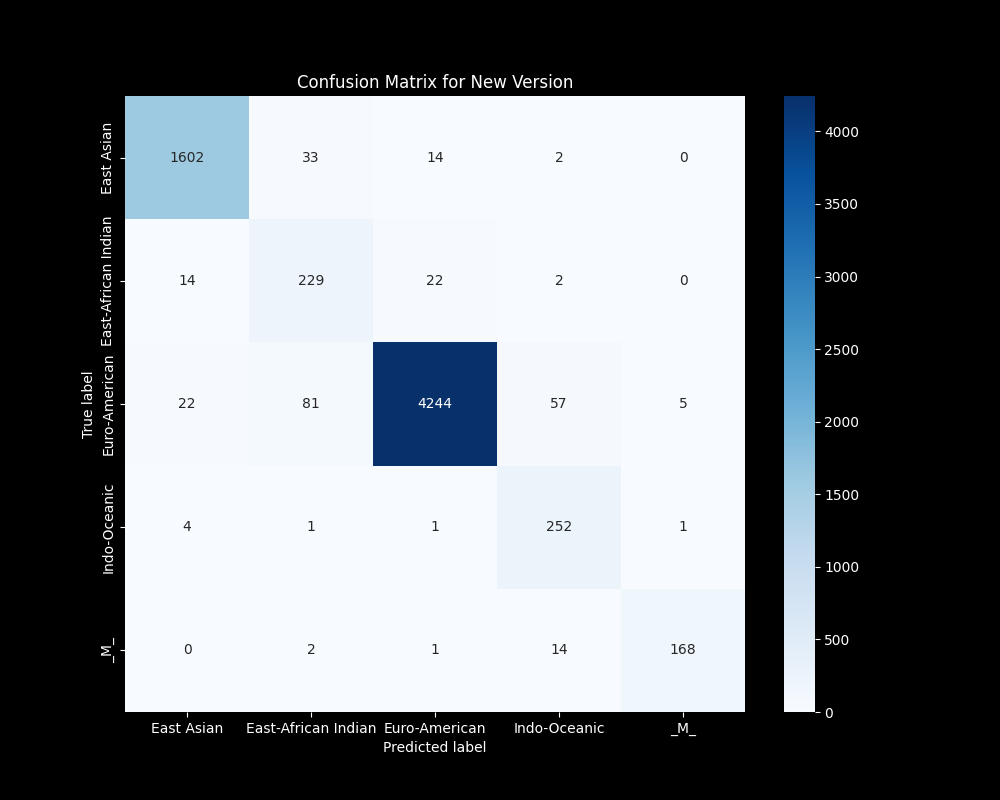
\includegraphics[width=0.65\textwidth]{../imgs/graphs/cnn_confusion_matrix_mosaics_100px.png}
		\caption{Confusion matrix on the mosaic images at 100px resolution without any additional techniques applied.}
		\label{fig:initial_confusion_matrix_mosaic}
	\end{figure}

	% ------ kfold cross validation ------
	\section{K-Fold Cross Validation}
	\label{app:kfold_cross_validation}

	\begin{figure}[H]
		\centering
		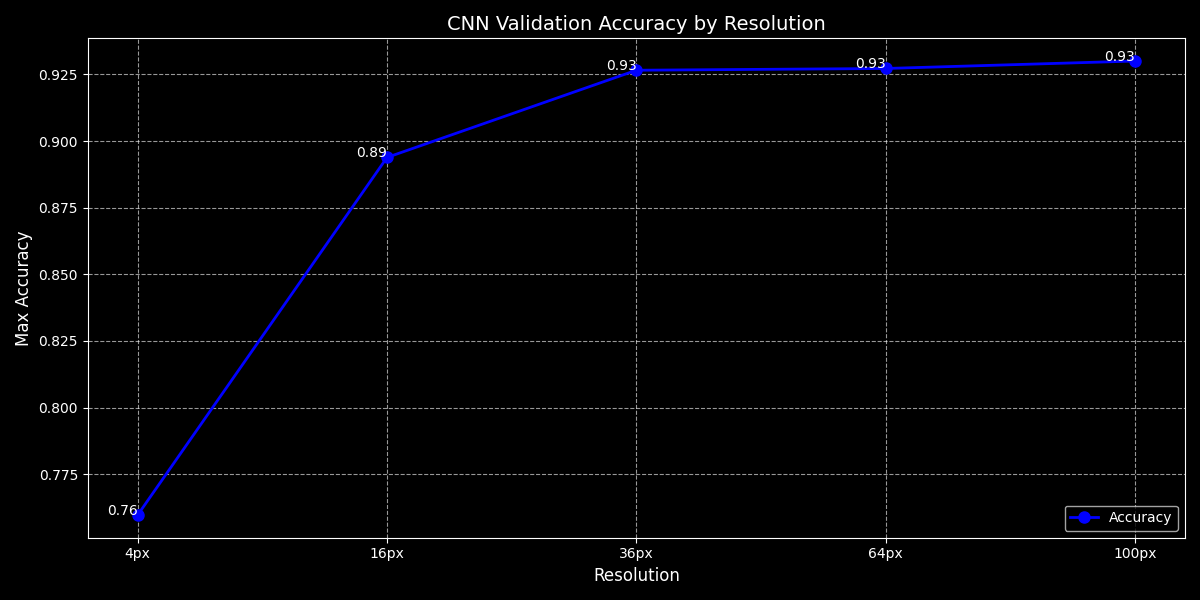
\includegraphics[width=0.65\textwidth]{../imgs/graphs/kfold/cnn_validation_accuracy_kfold_mosaics_line_mask_5_std.png}
		\caption{Graph showing the validation accuracy of the CNN model with k-fold cross validation applied on the mosaic images.}
		\label{fig:kfold_accuracy_mosaic}
	\end{figure}

	\begin{figure}[H]
		\centering
		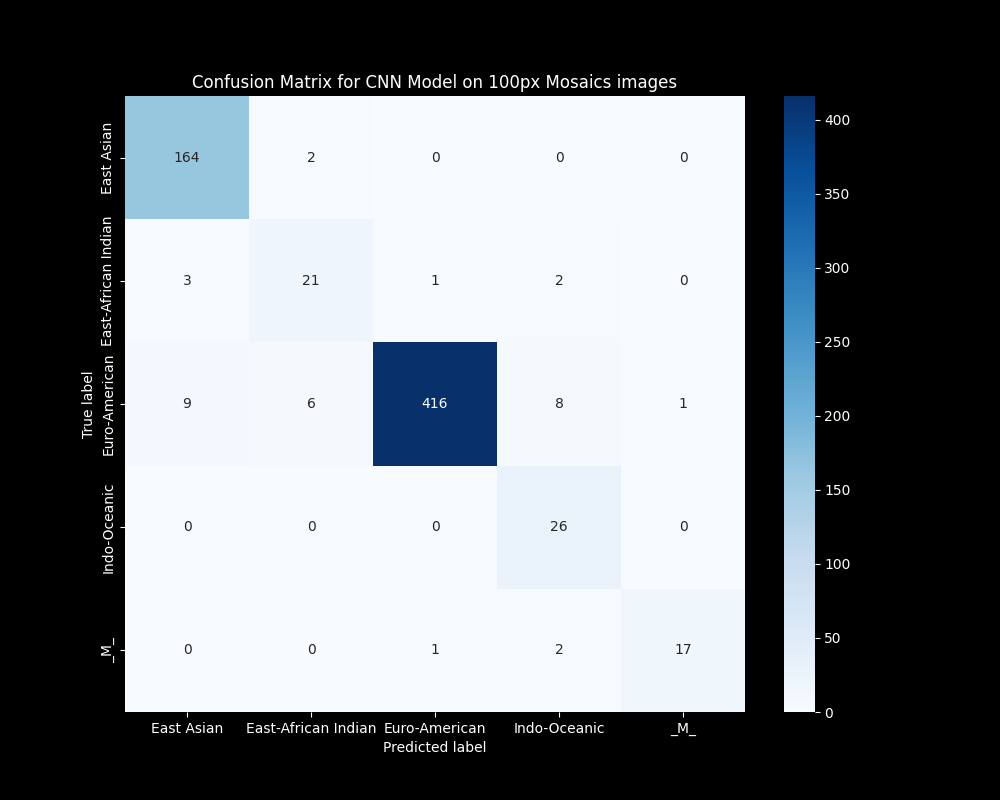
\includegraphics[width=0.65\textwidth]{../imgs/graphs/kfold/cnn_confusion_matrix_kfold_mosaics_100px_mask_5_std.png}
		\caption{Confusion matrix with k-fold cross validation applied on the mosaic images at 100px resolution.}
		\label{fig:kfold_confusion_matrix_mosaic}
	\end{figure}

	% ------ under-sampling ------
	\section{Under-Sampling techniques applied}
	\label{app:under_sampling}

	\begin{figure}[H]
		\centering
		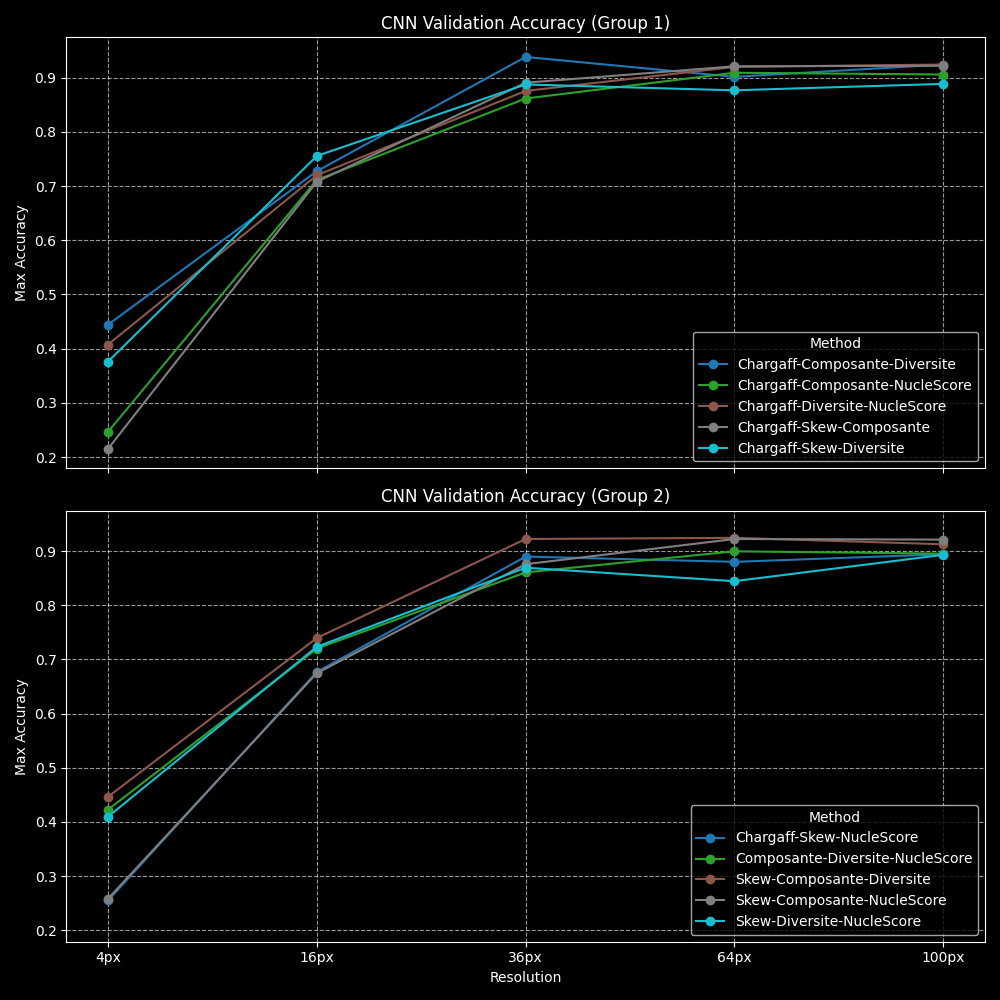
\includegraphics[width=0.7\textwidth]{../imgs/graphs/kfold-undersample/cnn_validation_accuracy_groups_mask_5_kfold_undersample.png}
		\caption{Graph showing the validation accuracy of the CNN model with under-sampling applied on the different methods.}
		\label{fig:under_sampling_accuracy}
	\end{figure}

	\begin{figure}[H]
		\centering
		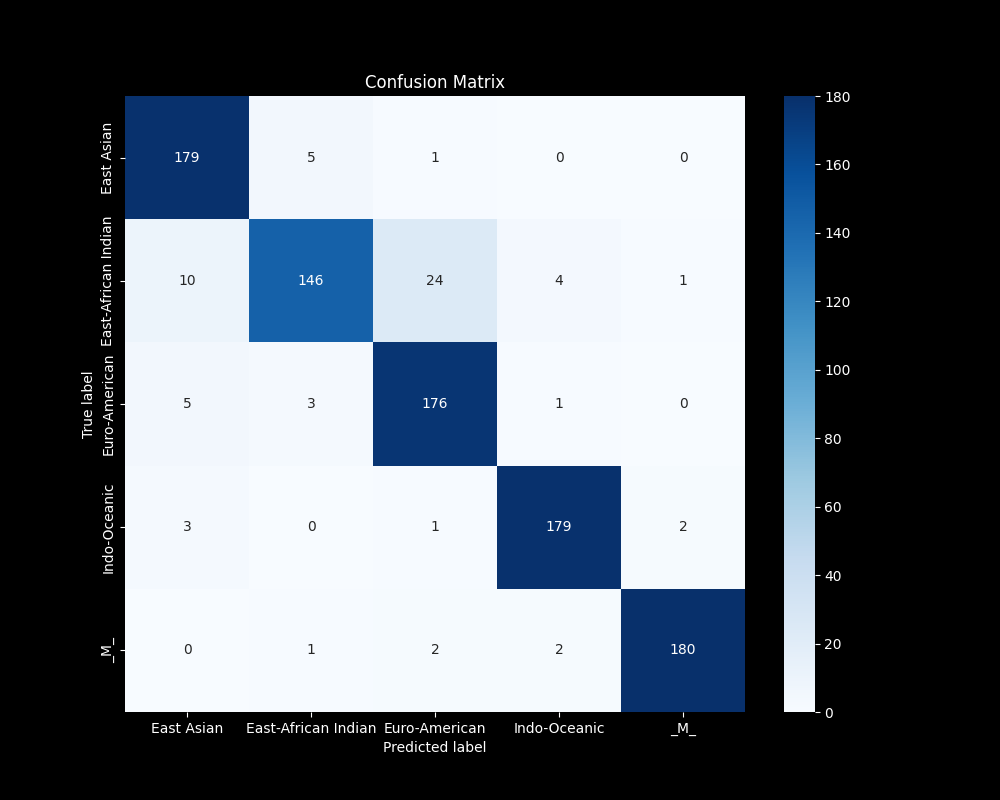
\includegraphics[width=0.7\textwidth]{../imgs/graphs/kfold-undersample/cnn_confusion_matrix_100px_mask_5-kfold_undersample.png}
		\caption{Confusion matrix with under-sampling applied on the images obtained from the Chargaff-Diversity-NucleScore
			combination at 100px resolution.}
		\label{fig:under_sampling_confusion_matrix}
	\end{figure}

	\begin{figure}[H]
		\centering
		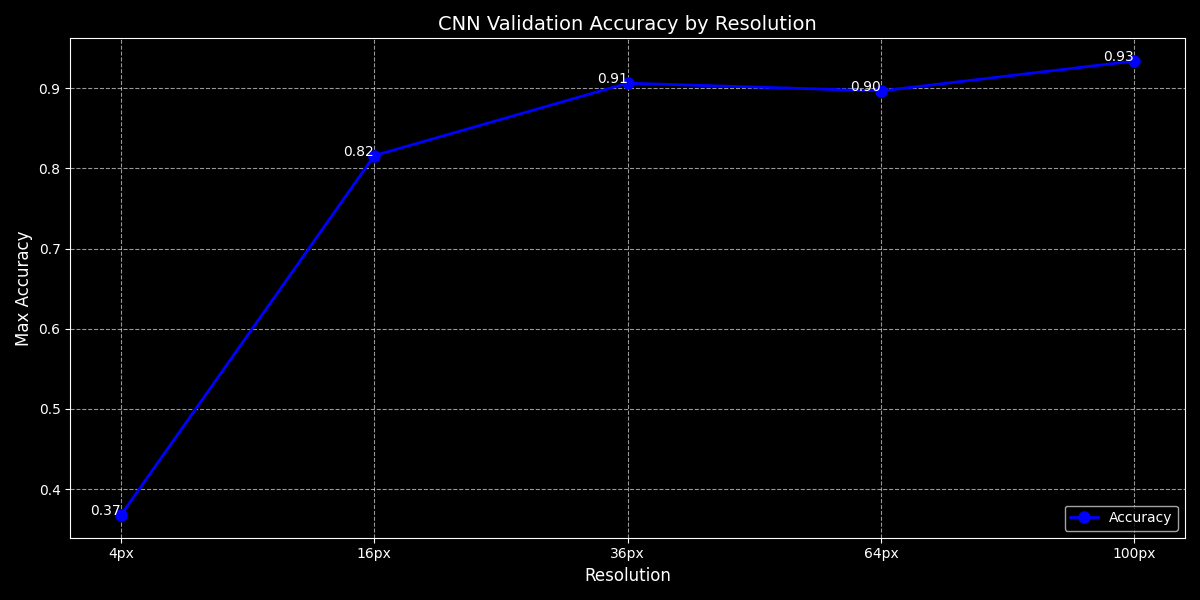
\includegraphics[width=0.7\textwidth]{../imgs/graphs/kfold-undersample/cnn_validation_accuracy_kfold_mosaics_line_mask_5_undersample.png}
		\caption{Graph showing the validation accuracy of the CNN model with under-sampling applied on the mosaic images.}
		\label{fig:under_sampling_mosaic_accuracy}
	\end{figure}

	\begin{figure}[H]
		\centering
		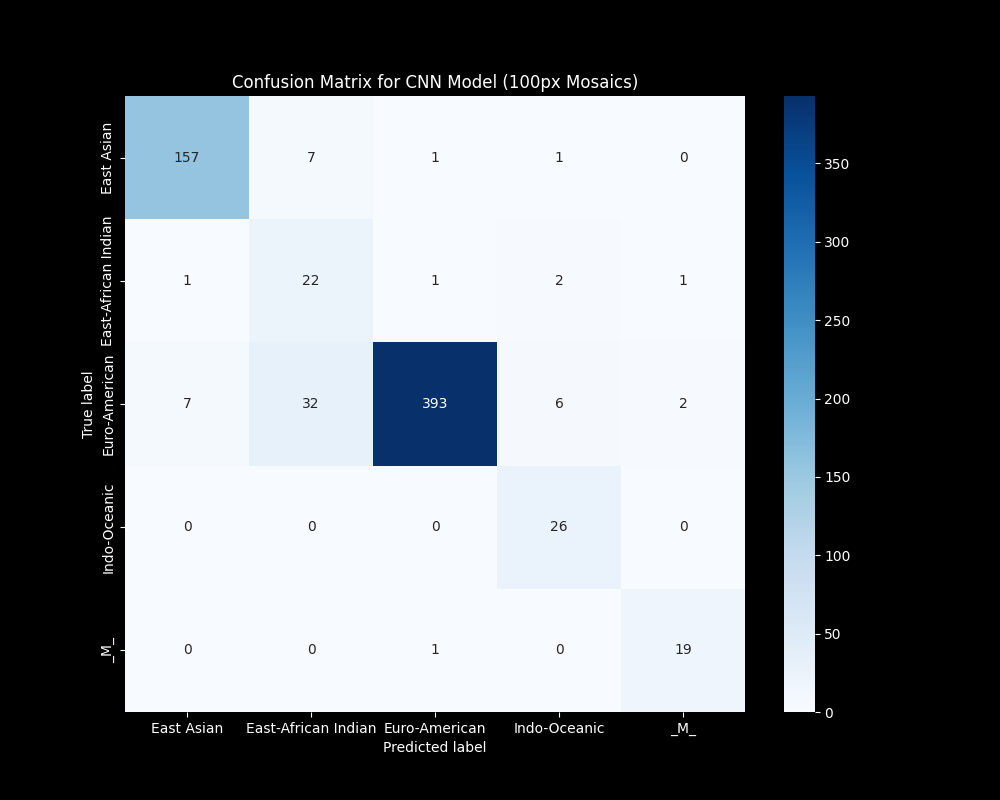
\includegraphics[width=0.7\textwidth]{../imgs/graphs/kfold-undersample/cnn_confusion_matrix_kfold_mosaics_100px_mask_5_undersample.png}
		\caption{Confusion matrix with under-sampling applied on the mosaic images at 100px resolution.}
		\label{fig:under_sampling_mosaic_confusion_matrix}
	\end{figure}

	% ------ data augmentation ------
	\section{Data Augmentation techniques applied}
	\label{app:data_augmentation}

	\begin{figure}[H]
		\centering
		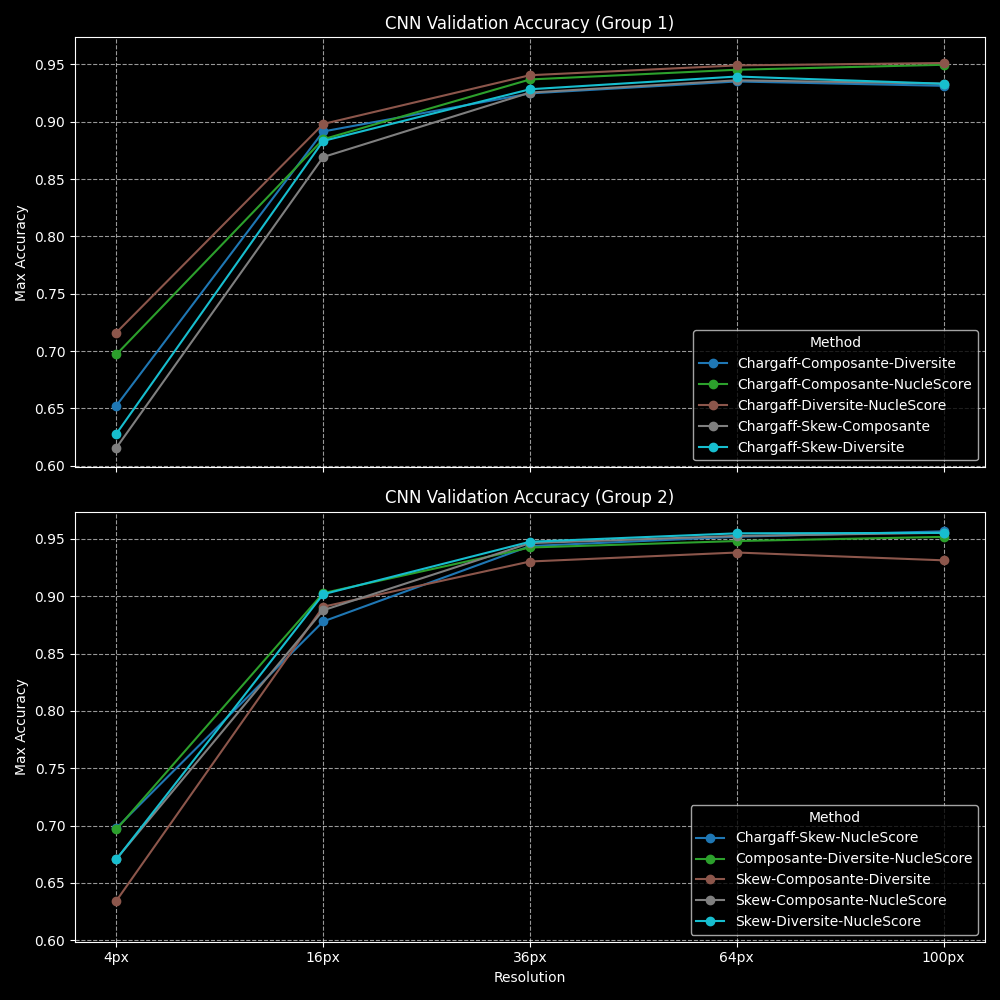
\includegraphics[width=0.7\textwidth]{../imgs/graphs/kfold/cnn_validation_accuracy_groups_mask_5_kfold_aug.png}
		\caption{Graph showing the validation accuracy of the CNN model with data augmentation applied on the different methods.}
		\label{fig:augmentation_accuracy}
	\end{figure}

	\begin{figure}[H]
		\centering
		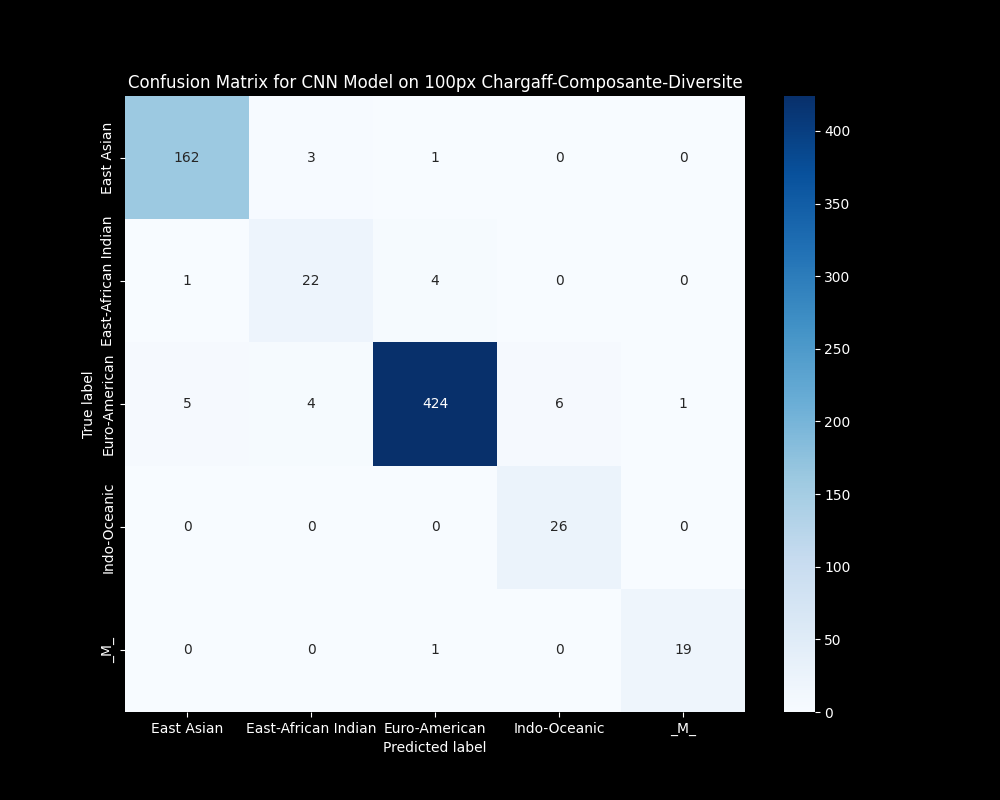
\includegraphics[width=0.7\textwidth]{../imgs/graphs/kfold/cnn_confusion_matrix_100px_mask_5-kfold_aug.png}
		\caption{Confusion matrix with data augmentation applied on the images obtained from the Chargaff-Diversity-NucleScore
			combination at 100px resolution.}
		\label{fig:augmentation_confusion_matrix}
	\end{figure}

	\begin{figure}[H]
		\centering
		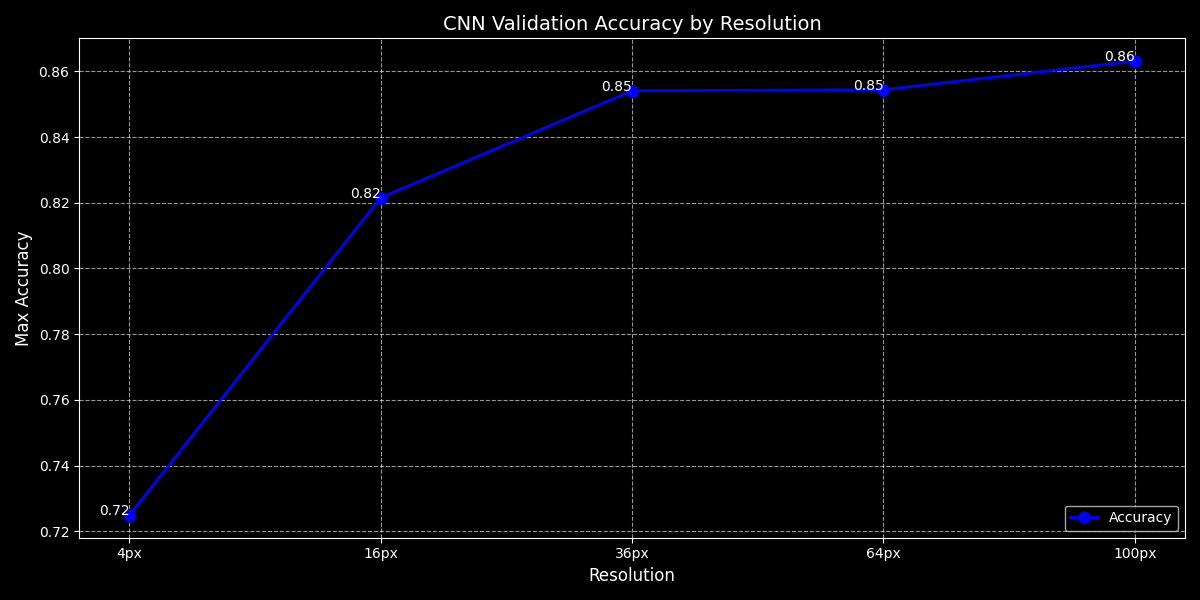
\includegraphics[width=0.7\textwidth]{../imgs/graphs/kfold/cnn_validation_accuracy_kfold_mosaics_line_mask_5_aug.png}
		\caption{Graph showing the validation accuracy of the CNN model with data augmentation applied on the mosaic images.}
		\label{fig:augmentation_accuracy_mosaic}
	\end{figure}

	\begin{figure}[H]
		\centering
		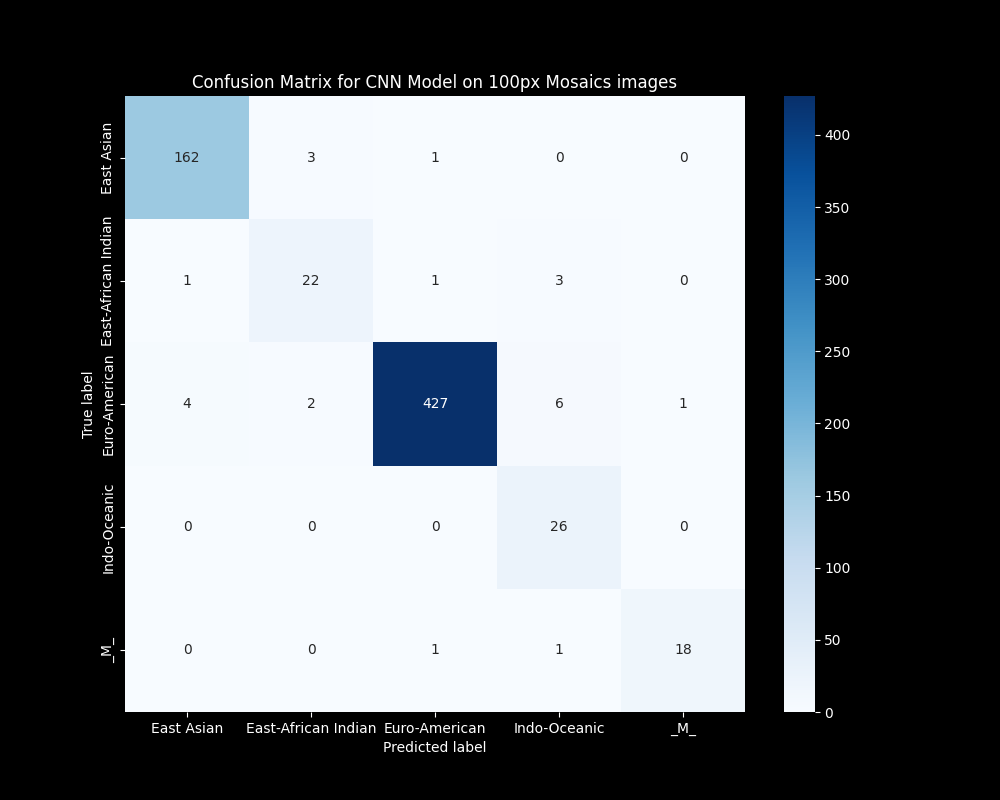
\includegraphics[width=0.7\textwidth]{../imgs/graphs/kfold/cnn_confusion_matrix_kfold_mosaics_100px_mask_5_aug.png}
		\caption{Confusion matrix with data augmentation applied on the mosaic images at 100px resolution.}
		\label{fig:augmentation_confusion_matrix_mosaic}
	\end{figure}

	% ------- combined techniques -------
	\section{Combined Techniques}
	\label{app:combined_techniques}

	\begin{figure}[H]
		\centering
		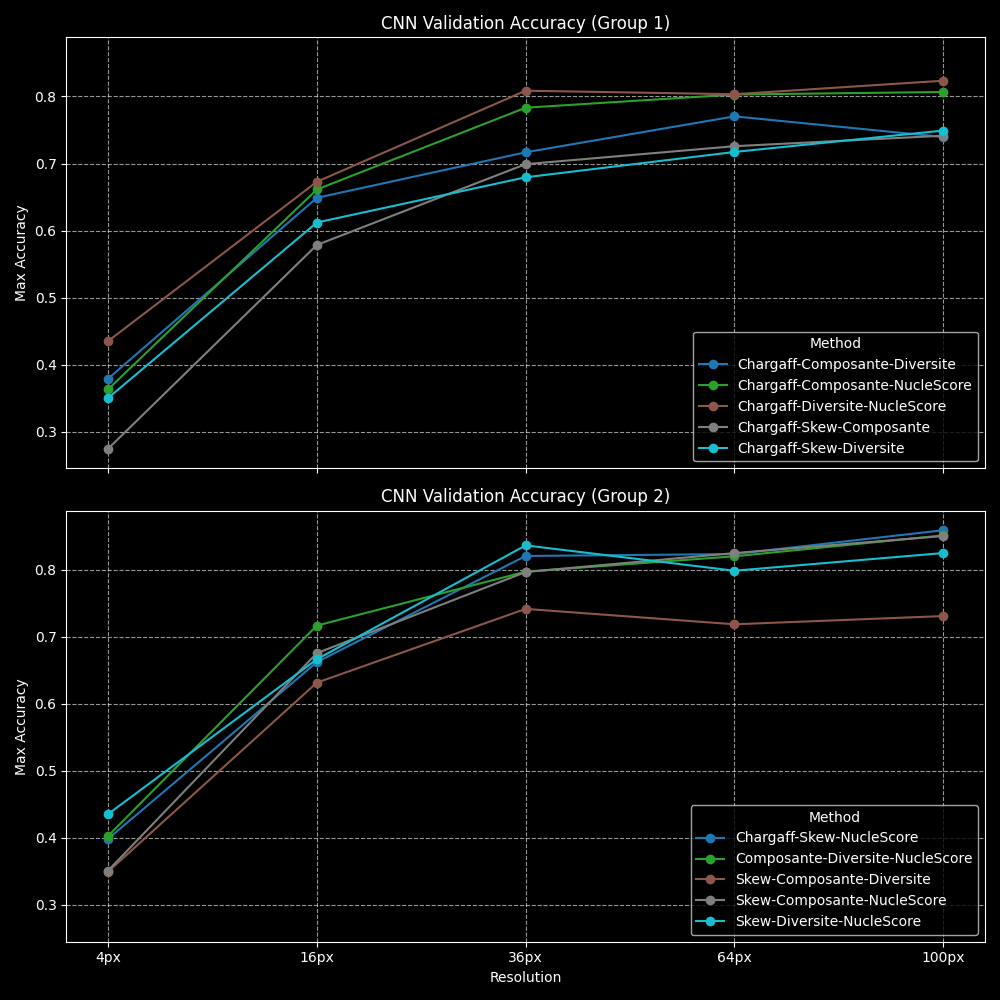
\includegraphics[width=0.7\textwidth]{../imgs/graphs/kfold-undersample/cnn_validation_accuracy_groups_mask_5_kfold_aug-under.png}
		\caption{Graph showing the validation accuracy of the CNN model with combined under-sampling and data augmentation
			techniques applied on the different methods.}
		\label{fig:combined_techniques_accuracy}
	\end{figure}

	\begin{figure}[H]
		\centering
		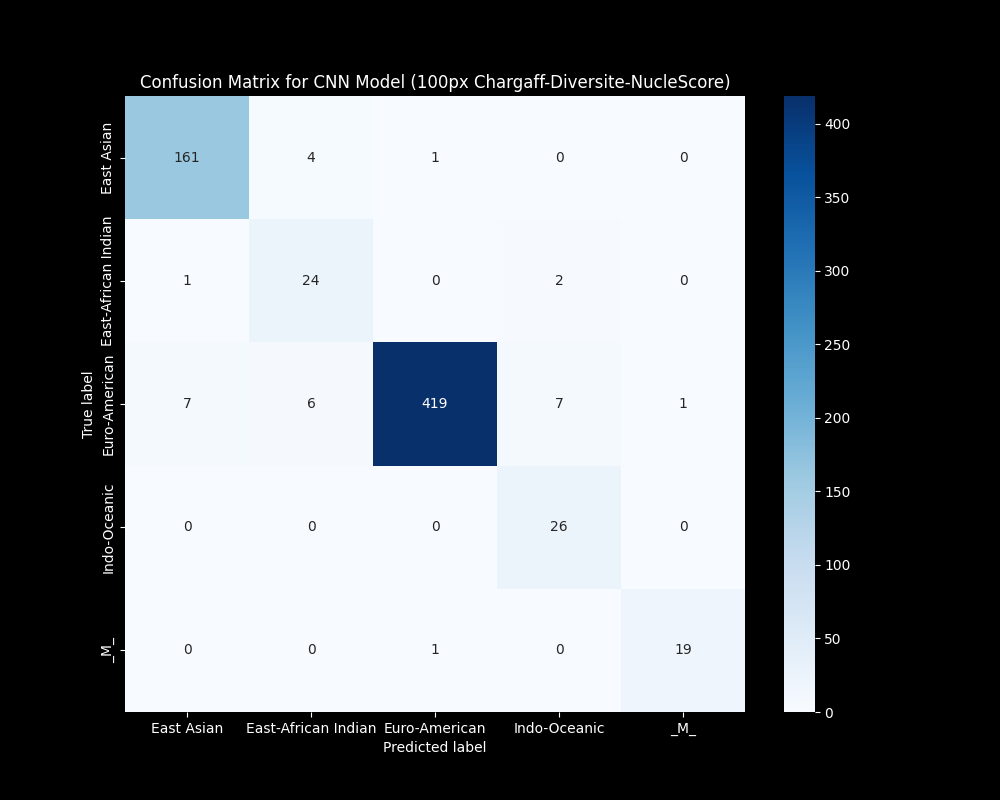
\includegraphics[width=0.7\textwidth]{../imgs/graphs/kfold-undersample/cnn_confusion_matrix_100px_mask_5-kfold_aug-under.png}
		\caption{Confusion matrix with combined under-sampling and data augmentation techniques
			applied on the images obtained from the Chargaff-Diversity-NucleScore combination at 100px resolution.}
		\label{fig:combined_techniques_confusion_matrix}
	\end{figure}

	\begin{figure}[H]
		\centering
		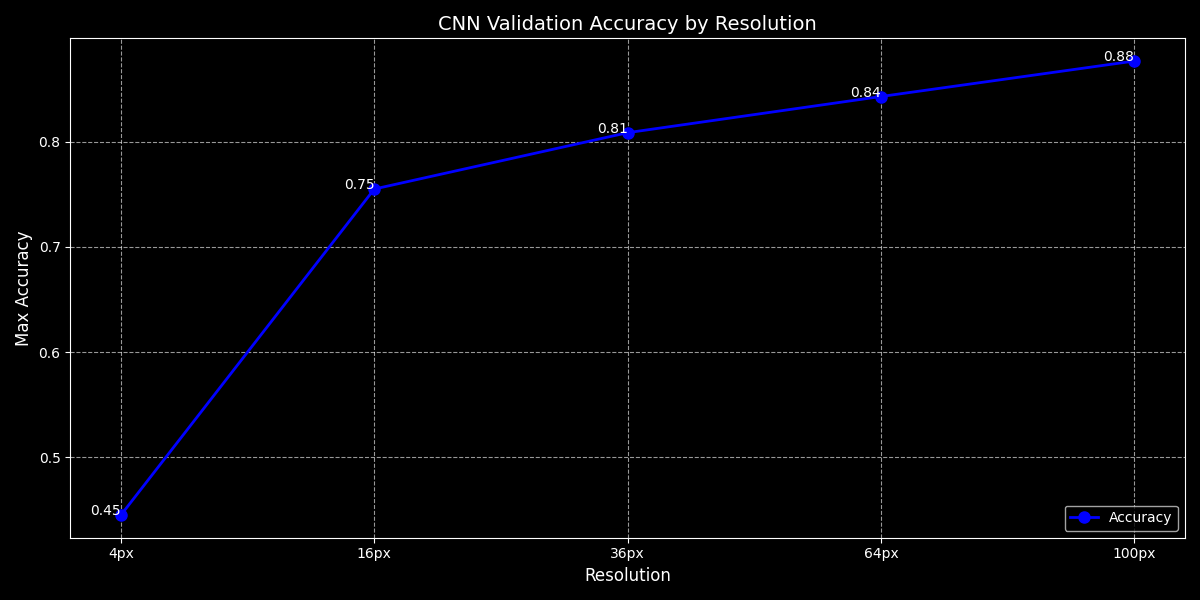
\includegraphics[width=0.7\textwidth]{../imgs/graphs/kfold-undersample/cnn_validation_accuracy_kfold_mosaics_line_mask_5_aug-under.png}
		\caption{Graph showing the validation accuracy of the CNN model with combined under-sampling and data augmentation
			techniques applied on the mosaic images.}
		\label{fig:combined_techniques_accuracy_mosaic}
	\end{figure}

	\begin{figure}[H]
		\centering
		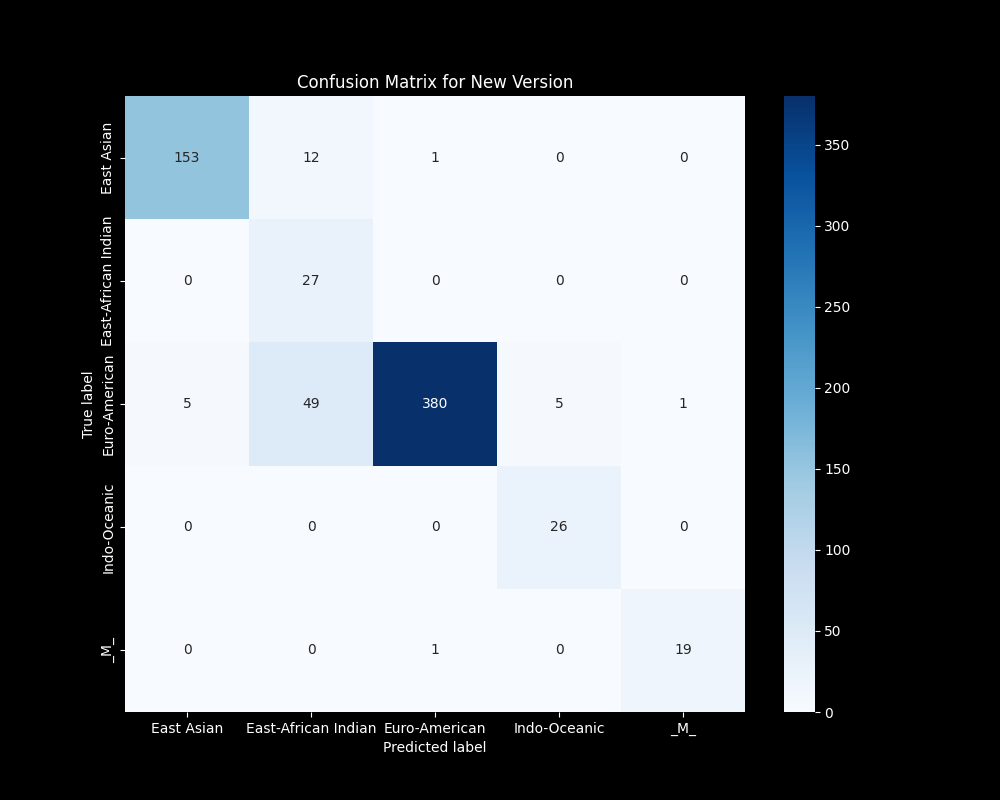
\includegraphics[width=0.7\textwidth]{../imgs/graphs/kfold-undersample/cnn_confusion_matrix_kfold_mosaics_100px_mask_5_aug-under.png}
		\caption{Confusion matrix with combined under-sampling and data augmentation techniques
			applied on the mosaic images at 100px resolution.}
		\label{fig:combined_techniques_confusion_matrix_mosaic}
	\end{figure}

\end{appendices}